\section{Method}
\label{sec:method}

The method combines the prioritized assignment and route-window procedures of the centralized baseline \cite{guo2024} with a hierarchical floor decomposition. A central server assigns jobs, splits routes at lifts, books lift trips, and merges plans; one edge server per floor plans local route legs.

Figure~\ref{fig:architecture} shows the information flow. Jobs and fleet state go to the central server; legs and reservations cross between central and floor servers; merged, verified schedules go to the AGVs for execution.

\subsection{Algorithms 1--3 recap}
Algorithm~\ref{alg:assignment} assigns jobs in order $(t_j,j)$ to the AGV minimizing $F_{ji}$. Algorithm~\ref{alg:routing} processes AGVs in priority order $V_1\to V_{|V|}$, constructing node and edge windows; a window conflicting with frozen reservations triggers Algorithm~\ref{alg:sliding}, which delays the affected route segment. Algorithm~\ref{alg:sliding} sweeps backward from the conflict visit to the nearest preceding exempt node, accumulating the smallest right-shift that clears higher-priority windows with separation $\delta$, up to $k_{\max}$ passes; on exhaustion it delays departure at the exempt node until blocking traffic clears.

\begin{algorithm}[t]
\caption{Prioritized job assignment (Algorithm 1)}
\label{alg:assignment}
\small
\begin{algorithmic}[1]
\REQUIRE Jobs $J$, AGVs $V$, fitness weight $\lambda$, service times $\eta,\eta'$
\ENSURE Assignment $x_{ji}$ and complete routes $R_i$
\FOR{each $j\in J$ in order $(t_j,j)$}
  \FOR{each $i\in V$}
    \STATE Compute $ct_{ji},et_{ji},dt_{ji}$ from AGV state $(s_i,vt_i)$.
    \STATE $F_{ji}\gets ct_{ji}+\lambda(et_{ji}+dt_{ji})$.
  \ENDFOR
  \STATE Choose $i^*\gets\arg\min_i(F_{ji},\rho_i)$; set $x_{ji^*}\gets1$.
  \STATE Append shortest paths $s_{i^*}\to p_j\to p'_j$ with dwell $\eta,\eta'$.
  \STATE Update AGV state to $(p'_j,ct_{ji^*})$.
\ENDFOR
\FOR{each $i\in V$}
  \STATE Append a shortest path from the final assigned station to $\pi$.
\ENDFOR
\end{algorithmic}
\end{algorithm}

\begin{algorithm}[t]
\caption{Prioritized conflict-free routing (Algorithm 2)}
\label{alg:routing}
\small
\begin{algorithmic}[1]
\REQUIRE Routes $R_i$, dwell times, priority order $V_1,\ldots,V_{|V|}$
\ENSURE Timed plans and frozen reservations $W_n,W'_e$
\STATE Initialize empty node and edge reservation sets $W_n,W'_e$.
\FOR{each AGV $i$ in priority order}
  \STATE Construct node and edge windows along $R_i$.
  \FOR{each candidate window conflicting with $W_n$ or $W'_e$}
    \STATE Apply Algorithm~\ref{alg:sliding} to delay the route segment.
  \ENDFOR
  \STATE Freeze ordinary node windows in $W_n$ and track windows in $W'_e$.
\ENDFOR
\end{algorithmic}
\end{algorithm}

\begin{algorithm}[t]
\caption{Sliding-window conflict elimination (Algorithm 3)}
\label{alg:sliding}
\small
\begin{algorithmic}[1]
\REQUIRE Conflict visit $p$, reservations $W$, route $R$, limit $k_{\max}$
\ENSURE Conflict-free shifted windows and delay $st^*$
\STATE Find the nearest preceding exempt visit $q$.
\FOR{$k=1$ to $k_{\max}$}
  \STATE Set $st^*\gets0$ and $mt^*\gets\infty$.
  \FOR{visits $m=p,p-1,\ldots,q+1$}
    \STATE Evaluate $f(lt_m+st^*,rt_m+st^*,W)$; update $mt^*$ and $st^*$.
    \IF{$st^*>mt^*$} \STATE Stop this backward sweep. \ENDIF
  \ENDFOR
  \IF{the sweep completes within $mt^*$} \STATE \textbf{break} \ENDIF
\ENDFOR
\IF{no feasible sweep completed}
  \STATE Apply the fallback delay at $q$ until blocking reservations clear.
\ENDIF
\STATE Shift windows $q+1,\ldots,p$ and extend the window at $q$ by $st^*$.
\end{algorithmic}
\end{algorithm}

\subsection{Hybrid central-plus-floor-server extension}
The hybrid planner cuts each complete route at lift edges into floor-local legs. Each floor server schedules its legs using local node and track reservations; when needed, the AGV waits at its entry lobby or at $\pi$. The central server reserves the lift track at the earliest available time after the AGV is ready, respecting safety separation, then releases the next floor leg at the arrival lobby. Floor and lift windows are merged into complete plans before independent verification.

Legs are dispatched either in priority order or first-come-first-served (FCFS): FCFS orders legs by release time, AGV priority, then leg index; priority order processes higher-priority AGVs' legs first and is used as a decomposition check. On the tested seeds, priority-order hybrid plans match the centralized-with-lobbies plans. Configuration C (the default hybrid) uses FCFS order.

\begin{algorithm}[t]
\caption{Hybrid floor-leg planning and lift booking}
\label{alg:hybrid}
\small
\begin{algorithmic}[1]
\REQUIRE Assigned routes, floor planners, central lift calendar, dispatch order
\ENSURE Merged complete AGV plans
\STATE Split each route into maximal floor-local legs at every lift.
\STATE Insert each initial leg into the dispatch queue using the chosen order.
\WHILE{the queue is nonempty}
  \STATE Remove the next leg and schedule it with its floor planner.
  \IF{the route continues on another floor}
    \STATE Reserve the intervening lift trip centrally.
    \STATE Release the next leg at the arrival lobby after lift travel.
  \ENDIF
\ENDWHILE
\STATE Merge floor-leg and lift windows; independently verify each plan.
\end{algorithmic}
\end{algorithm}

\begin{figure}[t]
\centering
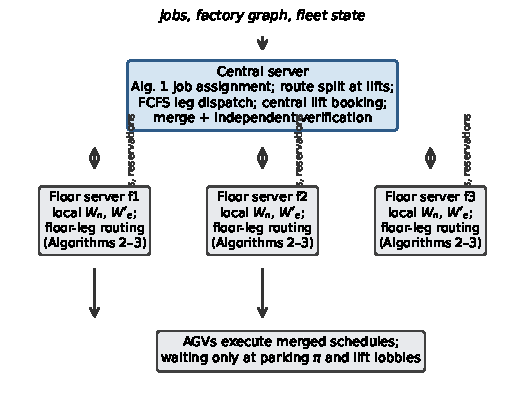
\includegraphics[width=\columnwidth]{../figures/architecture.pdf}
\caption{Hybrid architecture: central job assignment, route split, lift booking, and verification; per-floor route-leg planning; AGVs execute merged schedules, waiting only at parking $\pi$ and lift lobbies.}
\label{fig:architecture}
\end{figure}
